\documentclass[xcolor=svgnames]{beamer}\usepackage[]{graphicx}\usepackage[]{color}
%% maxwidth is the original width if it is less than linewidth
%% otherwise use linewidth (to make sure the graphics do not exceed the margin)
\makeatletter
\def\maxwidth{ %
  \ifdim\Gin@nat@width>\linewidth
    \linewidth
  \else
    \Gin@nat@width
  \fi
}
\makeatother

\definecolor{fgcolor}{rgb}{0.345, 0.345, 0.345}
\newcommand{\hlnum}[1]{\textcolor[rgb]{0.686,0.059,0.569}{#1}}%
\newcommand{\hlstr}[1]{\textcolor[rgb]{0.192,0.494,0.8}{#1}}%
\newcommand{\hlcom}[1]{\textcolor[rgb]{0.678,0.584,0.686}{\textit{#1}}}%
\newcommand{\hlopt}[1]{\textcolor[rgb]{0,0,0}{#1}}%
\newcommand{\hlstd}[1]{\textcolor[rgb]{0.345,0.345,0.345}{#1}}%
\newcommand{\hlkwa}[1]{\textcolor[rgb]{0.161,0.373,0.58}{\textbf{#1}}}%
\newcommand{\hlkwb}[1]{\textcolor[rgb]{0.69,0.353,0.396}{#1}}%
\newcommand{\hlkwc}[1]{\textcolor[rgb]{0.333,0.667,0.333}{#1}}%
\newcommand{\hlkwd}[1]{\textcolor[rgb]{0.737,0.353,0.396}{\textbf{#1}}}%

\usepackage{framed}
\makeatletter
\newenvironment{kframe}{%
 \def\at@end@of@kframe{}%
 \ifinner\ifhmode%
  \def\at@end@of@kframe{\end{minipage}}%
  \begin{minipage}{\columnwidth}%
 \fi\fi%
 \def\FrameCommand##1{\hskip\@totalleftmargin \hskip-\fboxsep
 \colorbox{shadecolor}{##1}\hskip-\fboxsep
     % There is no \\@totalrightmargin, so:
     \hskip-\linewidth \hskip-\@totalleftmargin \hskip\columnwidth}%
 \MakeFramed {\advance\hsize-\width
   \@totalleftmargin\z@ \linewidth\hsize
   \@setminipage}}%
 {\par\unskip\endMakeFramed%
 \at@end@of@kframe}
\makeatother

\definecolor{shadecolor}{rgb}{.97, .97, .97}
\definecolor{messagecolor}{rgb}{0, 0, 0}
\definecolor{warningcolor}{rgb}{1, 0, 1}
\definecolor{errorcolor}{rgb}{1, 0, 0}
\newenvironment{knitrout}{}{} % an empty environment to be redefined in TeX

\usepackage{alltt}
\usetheme{Boadilla}
\usecolortheme[named=SeaGreen]{structure}
\usepackage{graphicx}
\usepackage{breqn}
\usepackage{xcolor}
\usepackage{booktabs}
\usepackage{verbatim}
\usepackage{tikz}
\usepackage{lmodern}
\usetikzlibrary{shadows,arrows,positioning}
\definecolor{links}{HTML}{2A1B81}
\hypersetup{colorlinks,linkcolor=links,urlcolor=links}
\usepackage{pgfpages}

\tikzstyle{block} = [rectangle, draw, text width=9em, text centered, rounded corners, minimum height=3em, minimum width=7em, top color = white, bottom color=brown!30,  drop shadow]

\newcommand{\ShowSexpr}[1]{\texttt{{\char`\\}Sexpr\{#1\}}}

\newcommand{\Bigtxt}[1]{\textbf{\textit{#1}}}

% knitr setup


\IfFileExists{upquote.sty}{\usepackage{upquote}}{}
\begin{document}

\title[Introduction to R]{Introduction to R}

\author[M. Beck, T. O'Brien]{Marcus W. Beck\inst{1} \and Todd D. O'Brien\inst{2}}

\date{}

\institute[]{\inst{1} ORISE, USEPA NHEERL Gulf Ecology Division\\ Email: \href{mailto:beck.marcus@epa.gov}{beck.marcus@epa.gov} \and \inst{2} NOAA/NMFS Copepod Project\\ Email: \href{todd.obrien@noaa.gov}{todd.obrien@noaa.gov}}

%%%%%%
\begin{frame}
\vspace{0.3in}
\centerline{
\begin{tikzpicture}
  \node[drop shadow={shadow xshift=0ex,shadow yshift=0ex},fill=white,draw] at (0,0) {\includegraphics[width=0.9\textwidth]{bg_main.jpg}};
\end{tikzpicture}}
\titlepage
\end{frame}

%%%%%%
\begin{frame}{What you'll learn in this intro}
\begin{itemize}
\itemsep15pt
\item Course expectations and pre-worskhop materials
\item What is R?
\item What's possible with R?
\item R basics
\begin{itemize}
\item Installation
\item Command-line interface
\item Coding basics
\item Functions and objects
\item Data import and manipulation
\end{itemize}
\item Help!\\~\\
\end{itemize}
\end{frame}

%%%%%%
\begin{frame}{Course expectations}
The November 17$^{th}$ workshop will provide you with a set of tools for evaluating time series data from SWMP \\~\\
Preparation for the workshop:
\begin{itemize}
\item Review pre-workshop toolkit materials
\item Bring a computer with R version 3.0.0 or later
\item Optionally, install RStudio in addition to R
\item Have a basic proficiency using R, what this means:
\begin{itemize}
\item You do not have to be an expert!
\item Understand the basics of a command-line interface
\item Know how to open R, load a script, execute functions
\item Know how to save your work 
\end{itemize}
\item Install the `SWMPr' package after installing R
\end{itemize}
\end{frame}

%%%%%%
\begin{frame}{Course expectations}
This is not an R training workshop... \\~\\
...but we will be using R exclusively to handle SWMP data\\~\\
You will receive an overview of the theory behind time series analysis \\~\\
We will use an R package developed to work with SWMP data \\~\\
A package is a collection of functions written by others that can be installed within R\\~\\
This package can automatically handle common problems working with SWMP data and time series, it is designed to make your life easier! \\~\\
\end{frame}

%%%%%%
\begin{frame}{Course expectations}
The pre-workshop toolkit includes:
\begin{itemize}
\item R installation instructions - \textit{R\_install\_guide.pdf}
\item Intro to R (current document) - \textit{intro\_to\_R.pdf}
\item Basics of data analysis with R - \textit{r\_for\_data\_analysis.pdf}
\item Installing and working with the SWMPr package - \textit{intro\_to\_swmpr.pdf}\\~\\
\end{itemize}
The final item is optional as we will cover the content in the workshop, but you should have the SWMPr package installed prior to the 17th\\~\\
Please note that webinar attendees will have limited interaction with the instructors, although we will have moderators handling questions.
\end{frame}

%%%%%%
\begin{frame}{Course expectations}
Copies of all instructional materials will be made available on the course website: \href{http://copepod.org/nerrs-swmp-workshop/}{copepod.org/nerrs-swmp-workshop/}\\~\\
Physical attendees will also receive a flashdrive with the course materials \\~\\
The instructors can also be contacted with questions prior to the workshop:\\~\\
\begin{itemize}
\item For R questions including toolkit and installation - Marcus Beck, \href{mailto:beck.marcus@epa.gov}{beck.marcus@epa.gov}
\item For time series analysis questions - Todd O'Brien, \href{mailto:todd.obrien@noaa.gov}{todd.obrien@noaa.gov}
\end{itemize}
\end{frame}

%%%%%%
\begin{frame}[containsverbatim]{Course expectations}
Finally, the presentation materials combine content with R code and R output\\~\\
R code that can be executed will look like this:
\begin{knitrout}
\definecolor{shadecolor}{rgb}{0.969, 0.969, 0.969}\color{fgcolor}\begin{kframe}
\begin{alltt}
\hlcom{# here's some R code}
\hlkwd{rnorm}\hlstd{(}\hlnum{10}\hlstd{)}
\end{alltt}
\end{kframe}
\end{knitrout}
The output will look similar to this in R (without `\#\#'):
\begin{knitrout}
\definecolor{shadecolor}{rgb}{0.969, 0.969, 0.969}\color{fgcolor}\begin{kframe}
\begin{verbatim}
##  [1]  0.5  1.6 -0.4 -0.9  0.5  0.8  1.5  0.7 -0.4  1.3
\end{verbatim}
\end{kframe}
\end{knitrout}
When applicable, R scripts are provided that contain only the executable code within each training module.  You can use these in R as you read each presentation.
\end{frame}

%%%%%%
\begin{frame}{What is \includegraphics[width=0.07\textwidth]{Rlogo.jpg} \hspace{0.2em}? }
R is a computer language that allows the user to program algorithms and use tools that have been programmed by others\\~\\
Different from other statistics software because it provides both tools for analysis and it is also a programming language...\\~\\
You do not have to be a progammer to use R!
\end{frame}

%%%%%%
\begin{frame}{What is \includegraphics[width=0.07\textwidth]{Rlogo.jpg} \hspace{0.2em}? }

\begin{center}
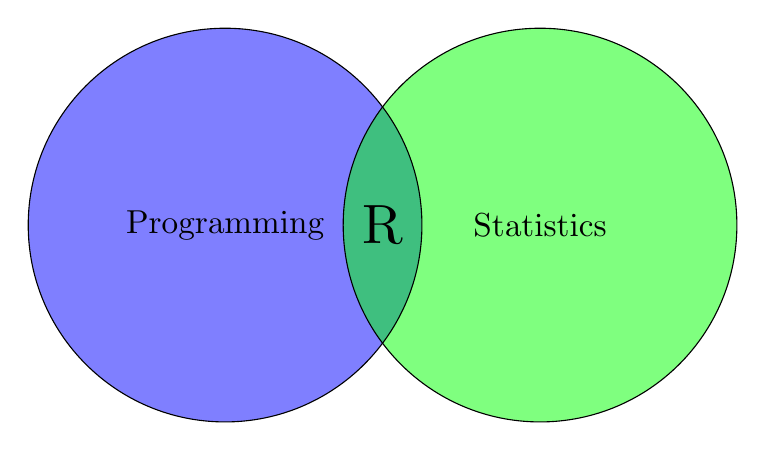
\begin{tikzpicture}
  \begin{scope}

    % The transparency:
    \begin{scope}[fill opacity=0.5]
      \fill[blue] (-2,0) circle (2.5);
      \fill[green] (2,0) circle (2.5);
    \end{scope}
    
    % letterings and missing pieces:
    \draw[align=center] (-2,0) circle (2.5) node[scale=1.2] {Programming};
    \draw[align=center] (2,0) circle (2.5) node[scale=1.2] {Statistics};
 		\draw (0,0) node[scale=2] {R};
 		
  \end{scope}
\end{tikzpicture}\\~\\
R is both... this creates a steep learning curve.
\end{center}
\end{frame}

%%%%%%
\begin{frame}[t]{What is \includegraphics[width=0.07\textwidth]{Rlogo.jpg} \hspace{0.2em}? }
\vspace{-0.1in}
\begin{columns}
\begin{column}{0.4\textwidth}
R is becoming the statistical software of choice\\~\\
Plot of Google scholar hits over time for different software packages
[\href{http://r4stats.com/articles/popularity/}{r4stats.com}]
\end{column}
\begin{column}{0.5\textwidth}
\begin{center}
\includegraphics[width=1.1\textwidth]{r_google.png}
\end{center}
\end{column}
\end{columns}
\end{frame}

%%%%%%
\begin{frame}[t]{What is \includegraphics[width=0.07\textwidth]{Rlogo.jpg} \hspace{0.2em}? }
\vspace{-0.1in}
\begin{columns}
\begin{column}{0.4\textwidth}
R is becoming the statistical software of choice\\~\\
Exponential growth in number of contributed packages
[\href{http://r4stats.com/articles/popularity/}{r4stats.com}]
\end{column}
\begin{column}{0.5\textwidth}
\begin{center}
\includegraphics[width=1.1\textwidth]{r_package.png}
\end{center}
\end{column}
\end{columns}
\end{frame}

%%%%%%
\begin{frame}{What's possible with \includegraphics[width=0.07\textwidth]{Rlogo.jpg} \hspace{0.2em}? }
R is incredibly flexible, if you want something done, someone else has written the code...\\~\\
R is open-source software, which mean it's free and is supported by a large network of contributors - the Comprehensive R Network [\href{http://cran.us.r-project.org/}{CRAN}]\\~\\
CRAN is a collection of sites which carry identical material, consisting of the R distribution(s), the contributed extensions, documentation for R, and binaries [\href{http://cran.us.r-project.org/faqs.html}{R FAQ}]\\~\\
Basically a repository of R utilities that others have written as well as the source files for R - the \href{http://cran.r-project.org/web/views/}{CRAN task views} contain descriptions of contributed packages by category
\end{frame}

%%%%%%
\begin{frame}[t]{What's possible with \includegraphics[width=0.07\textwidth]{Rlogo.jpg} \hspace{0.2em}? }
\href{http://cran.r-project.org/web/views/}{CRAN task views}
\begin{center}
\includegraphics[width = 0.8\textwidth]{cran_view1.png}
\end{center}
\end{frame}

%%%%%%
\begin{frame}[t]{What's possible with \includegraphics[width=0.07\textwidth]{Rlogo.jpg} \hspace{0.2em}? }
\href{https://github.com/}{Github} has also been increasingly used to store packages online  - like an informal CRAN:
\begin{center}
\includegraphics[width = 0.8\textwidth]{git.png}
\end{center}
\end{frame}

%%%%%%
\begin{frame}[t,fragile]{What's possible with \includegraphics[width=0.07\textwidth]{Rlogo.jpg} \hspace{0.2em}? }
R comes with a base package that is included in installation, others are downloaded as needed, e.g.,\\~\\
\begin{knitrout}
\definecolor{shadecolor}{rgb}{0.969, 0.969, 0.969}\color{fgcolor}\begin{kframe}
\begin{alltt}
\hlcom{# download from CRAN}
\hlkwd{install.packages}\hlstd{(}\hlstr{'ggplot2'}\hlstd{)}
\end{alltt}
\end{kframe}
\end{knitrout}
\vspace{0.2in}
The base package will be sufficient for most of your needs - includes arithmetic, input/output, basic programming support, graphics, etc.\\~\\
Once a package is installed, it must be loaded to use its functions:
\begin{knitrout}
\definecolor{shadecolor}{rgb}{0.969, 0.969, 0.969}\color{fgcolor}\begin{kframe}
\begin{alltt}
\hlcom{# load ggplot2}
\hlkwd{library}\hlstd{(ggplot2)}
\end{alltt}
\end{kframe}
\end{knitrout}
\end{frame}

%%%%%%
\begin{frame}[t,fragile]{What's possible with \includegraphics[width=0.07\textwidth]{Rlogo.jpg} \hspace{0.2em}? }
Or you can download packages from Github, which requires using the devtools package:
\begin{knitrout}
\definecolor{shadecolor}{rgb}{0.969, 0.969, 0.969}\color{fgcolor}\begin{kframe}
\begin{alltt}
\hlcom{# download devtools from CRAN}
\hlkwd{install.package}\hlstd{(}\hlstr{'devtools'}\hlstd{)}

\hlcom{# load devtools}
\hlkwd{library}\hlstd{(devtools)}

\hlcom{# install SWMPr from Github, load}
\hlkwd{install_github}\hlstd{(}\hlstr{'fawda123/SWMPr'}\hlstd{)}
\hlkwd{library}\hlstd{(SWMPr)}
\end{alltt}
\end{kframe}
\end{knitrout}
\end{frame}

%%%%%%
\begin{frame}[t,fragile]{What's possible with \includegraphics[width=0.07\textwidth]{Rlogo.jpg} \hspace{0.2em}? }
Each package may also come with a demonstration\\~\\
This provides a neat way to see what an R package has to offer\\~\\
To see a list of packages with demonstrations, run this code:
\begin{knitrout}
\definecolor{shadecolor}{rgb}{0.969, 0.969, 0.969}\color{fgcolor}\begin{kframe}
\begin{alltt}
\hlcom{# view packages with demos}
\hlkwd{demo}\hlstd{(}\hlkwc{package} \hlstd{=} \hlkwd{.packages}\hlstd{(}\hlkwc{all.available} \hlstd{=} \hlnum{TRUE}\hlstd{))}
\end{alltt}
\end{kframe}
\end{knitrout}
To view a demonstration of basic graphic capabilities in R:
\begin{knitrout}
\definecolor{shadecolor}{rgb}{0.969, 0.969, 0.969}\color{fgcolor}\begin{kframe}
\begin{alltt}
\hlcom{# view a demo for the graphics package}
\hlkwd{demo}\hlstd{(graphics)}
\end{alltt}
\end{kframe}
\end{knitrout}
\end{frame}

%%%%%%
\begin{frame}[t,fragile]{What's possible with \includegraphics[width=0.07\textwidth]{Rlogo.jpg} \hspace{0.2em}? }
Each package comes with extensive help documentation\\~\\
Help files for a package:
\begin{knitrout}
\definecolor{shadecolor}{rgb}{0.969, 0.969, 0.969}\color{fgcolor}\begin{kframe}
\begin{alltt}
\hlcom{# view help files for a package}
\hlkwd{help}\hlstd{(}\hlkwc{package} \hlstd{=} \hlstr{'ggplot2'}\hlstd{)}
\end{alltt}
\end{kframe}
\end{knitrout}
Or for an individual function in a package:
\begin{knitrout}
\definecolor{shadecolor}{rgb}{0.969, 0.969, 0.969}\color{fgcolor}\begin{kframe}
\begin{alltt}
\hlcom{# get help file}
\hlkwd{help}\hlstd{(mean,} \hlkwc{package} \hlstd{=} \hlstr{'base'}\hlstd{)}

\hlcom{# or do this}
\hlopt{?}\hlstd{mean}
\end{alltt}
\end{kframe}
\end{knitrout}
\end{frame}


\section{Basics}
%%%%%%
\begin{frame}[t]{\includegraphics[width=0.07\textwidth]{Rlogo.jpg} \hspace{0.01in} basics}
Following the instructions in our installation guide for step-by-step directions \\~\\
Or visit \href{http://cran.us.r-project.org/}{r-project.org} and follow directions
\centerline{\includegraphics[width = 0.8\textwidth]{download.png}}
\end{frame}

%%%%%%
\begin{frame}[t]{\includegraphics[width=0.07\textwidth]{Rlogo.jpg} \hspace{0.01in} basics}
\href{http://www.rstudio.com/}{RStudio} is also recommended but not required\\~\\
\centerline{\includegraphics[width=0.65\textwidth]{Rstudio.png}}
\end{frame}

%%%%%%
\begin{frame}[t]{\includegraphics[width=0.07\textwidth]{Rlogo.jpg} \hspace{0.01in} basics}
How is R different from Excel? R is a command-line interface\\~\\
\centerline{\includegraphics[width=0.7\textwidth]{command_line.png}}
\centerline{\emph{What next??}}
\end{frame}

%%%%%%
\begin{frame}[fragile]{\includegraphics[width=0.07\textwidth]{Rlogo.jpg} \hspace{0.01in} basics}
Lines of code are executed by R at the prompt (\textit{\texttt{>}})\\~\\
Enter the code and press enter, the output is returned
\begin{knitrout}
\definecolor{shadecolor}{rgb}{0.969, 0.969, 0.969}\color{fgcolor}\begin{kframe}
\begin{alltt}
\hlkwd{print}\hlstd{(}\hlstr{'hello world!'}\hlstd{)}
\end{alltt}
\begin{verbatim}
## [1] "hello world!"
\end{verbatim}
\begin{alltt}
\hlnum{2} \hlopt{+} \hlnum{2}
\end{alltt}
\begin{verbatim}
## [1] 4
\end{verbatim}
\begin{alltt}
\hlstd{(}\hlnum{2} \hlopt{+} \hlnum{2}\hlstd{)} \hlopt{/} \hlnum{4}
\end{alltt}
\begin{verbatim}
## [1] 1
\end{verbatim}
\end{kframe}
\end{knitrout}
\end{frame}

%%%%%%
\begin{frame}[fragile]{\includegraphics[width=0.07\textwidth]{Rlogo.jpg} \hspace{0.01in} basics}
A disadvantage of code is that everything entered must be 100 \% correct
\begin{knitrout}
\definecolor{shadecolor}{rgb}{0.969, 0.969, 0.969}\color{fgcolor}\begin{kframe}
\begin{alltt}
\hlnum{2} \hlopt{+} \hlstd{a}
\end{alltt}


{\ttfamily\noindent\bfseries\color{errorcolor}{\#\# Error: object 'a' not found}}\begin{alltt}
\hlstd{a}
\end{alltt}


{\ttfamily\noindent\bfseries\color{errorcolor}{\#\# Error: object 'a' not found}}\end{kframe}
\end{knitrout}
\vspace{0.2in}
But this provides an explicit documentation of your workflow...\\~\\
...your code is a living document of your analyses.
\end{frame}

%%%%%%
\begin{frame}[t,fragile]{\includegraphics[width=0.07\textwidth]{Rlogo.jpg} \hspace{0.01in} basics}
Assigning data to R objects is critical for analysis\\~\\
Assignment is possible using \textit{\texttt{<-}} or \textit{\texttt{=}}
\begin{knitrout}
\definecolor{shadecolor}{rgb}{0.969, 0.969, 0.969}\color{fgcolor}\begin{kframe}
\begin{alltt}
\hlstd{a} \hlkwb{<-} \hlnum{1}
\hlnum{2} \hlopt{+} \hlstd{a}
\end{alltt}
\begin{verbatim}
## [1] 3
\end{verbatim}
\begin{alltt}
\hlstd{a} \hlkwb{=} \hlnum{1}
\hlnum{2} \hlopt{+} \hlstd{a}
\end{alltt}
\begin{verbatim}
## [1] 3
\end{verbatim}
\end{kframe}
\end{knitrout}
\end{frame}

%%%%%%
\begin{frame}[t,fragile]{\includegraphics[width=0.07\textwidth]{Rlogo.jpg} \hspace{0.01in} basics}
More complex assignments are possible\\~\\
\begin{knitrout}
\definecolor{shadecolor}{rgb}{0.969, 0.969, 0.969}\color{fgcolor}\begin{kframe}
\begin{alltt}
\hlstd{a} \hlkwb{<-} \hlkwd{c}\hlstd{(}\hlnum{1}\hlstd{,} \hlnum{2}\hlstd{,} \hlnum{3} \hlstd{,} \hlnum{4}\hlstd{)}
\hlstd{a}
\end{alltt}
\begin{verbatim}
## [1] 1 2 3 4
\end{verbatim}
\begin{alltt}
\hlstd{a} \hlkwb{<-} \hlkwd{seq}\hlstd{(}\hlnum{1}\hlstd{,} \hlnum{4}\hlstd{)}
\hlstd{a}
\end{alltt}
\begin{verbatim}
## [1] 1 2 3 4
\end{verbatim}
\begin{alltt}
\hlstd{a} \hlkwb{<-} \hlkwd{c}\hlstd{(}\hlstr{'a'}\hlstd{,} \hlstr{'b'}\hlstd{,} \hlstr{'c'}\hlstd{)}
\hlstd{a}
\end{alltt}
\begin{verbatim}
## [1] "a" "b" "c"
\end{verbatim}
\end{kframe}
\end{knitrout}
\end{frame}

%%%%%%
\begin{frame}[fragile]{\includegraphics[width=0.07\textwidth]{Rlogo.jpg} \hspace{0.01in} basics}
Anatomy of a function - functions perform tasks for you, much like in Excel
\begin{center}
\Large
function(arguments)
\end{center}
\begin{knitrout}
\definecolor{shadecolor}{rgb}{0.969, 0.969, 0.969}\color{fgcolor}\begin{kframe}
\begin{alltt}
\hlkwd{c}\hlstd{(}\hlnum{1}\hlstd{,} \hlnum{2}\hlstd{)} \hlcom{# concatenate function to combine value}
\end{alltt}
\begin{verbatim}
## [1] 1 2
\end{verbatim}
\begin{alltt}
\hlkwd{mean}\hlstd{(}\hlkwd{c}\hlstd{(}\hlnum{1}\hlstd{,} \hlnum{2}\hlstd{))} \hlcom{# mean function}
\end{alltt}
\begin{verbatim}
## [1] 2
\end{verbatim}
\begin{alltt}
\hlkwd{seq}\hlstd{(}\hlnum{1}\hlstd{,} \hlnum{4}\hlstd{)} \hlcom{# create a sequence of values}
\end{alltt}
\begin{verbatim}
## [1] 1 2 3 4
\end{verbatim}
\end{kframe}
\end{knitrout}
\end{frame}

%%%%%%
\begin{frame}[fragile,t]{\includegraphics[width=0.07\textwidth]{Rlogo.jpg} \hspace{0.01in} basics}
Understanding classes of R \href{http://cran.r-project.org/doc/manuals/r-release/R-lang.html#Vector-objects}{objects} is necessary for analysis \\~\\
An object is a variable of interest that will always have a class\\~\\
Most common are `numeric' or `character' classes \\~\\
\begin{knitrout}
\definecolor{shadecolor}{rgb}{0.969, 0.969, 0.969}\color{fgcolor}\begin{kframe}
\begin{alltt}
\hlkwd{class}\hlstd{(}\hlnum{1}\hlstd{)}
\end{alltt}
\begin{verbatim}
## [1] "numeric"
\end{verbatim}
\begin{alltt}
\hlkwd{class}\hlstd{(}\hlstr{'1'}\hlstd{)}
\end{alltt}
\begin{verbatim}
## [1] "character"
\end{verbatim}
\end{kframe}
\end{knitrout}
`Factors' are also common, define categorical variables
\end{frame}

%%%%%%
\begin{frame}[fragile,t]{\includegraphics[width=0.07\textwidth]{Rlogo.jpg} \hspace{0.01in} basics}
Different types of methods are assigned to different class types\\~\\
The class also imposes limits on how it interacts with other class \\~\\
For example, we cannot add add two objects with different classes:\\~\\
\begin{knitrout}
\definecolor{shadecolor}{rgb}{0.969, 0.969, 0.969}\color{fgcolor}\begin{kframe}
\begin{alltt}
\hlcom{# this does not work}
\hlstr{'1'} \hlopt{+} \hlnum{1}
\end{alltt}


{\ttfamily\noindent\bfseries\color{errorcolor}{\#\# Error: non-numeric argument to binary operator}}\end{kframe}
\end{knitrout}
There is no `addition' method for character objects...
\end{frame}

%%%%%%
\begin{frame}[fragile]{\includegraphics[width=0.07\textwidth]{Rlogo.jpg} \hspace{0.01in} basics}
Objects (and their classes) are stored in the computer's memory in different ways - aka the workspace for your R session\\~\\
The most common structures are `vectors' and `data.frames'\\~\\
Vectors are a collection of objects of the same class, whereas a data frame is analogous to a table with rows and columns (e.g., collection of vectors)
\vspace{-0.2in}
\begin{columns}[t]
\begin{column}{0.5\textwidth}
\begin{knitrout}
\definecolor{shadecolor}{rgb}{0.969, 0.969, 0.969}\color{fgcolor}\begin{kframe}
\begin{alltt}
\hlstd{a} \hlkwb{<-} \hlkwd{c}\hlstd{(}\hlnum{1}\hlstd{,}\hlnum{2}\hlstd{)} \hlcom{# numeric vector}
\hlstd{a}
\end{alltt}
\begin{verbatim}
## [1] 1 2
\end{verbatim}
\begin{alltt}
\hlstd{b} \hlkwb{<-} \hlkwd{c}\hlstd{(}\hlstr{'a'}\hlstd{,} \hlstr{'b'}\hlstd{)} \hlcom{# character}
\hlstd{b}
\end{alltt}
\begin{verbatim}
## [1] "a" "b"
\end{verbatim}
\end{kframe}
\end{knitrout}
\end{column}
\begin{column}{0.5\textwidth}
\begin{knitrout}
\definecolor{shadecolor}{rgb}{0.969, 0.969, 0.969}\color{fgcolor}\begin{kframe}
\begin{alltt}
\hlcom{# data frame with both}
\hlstd{c} \hlkwb{<-} \hlkwd{data.frame}\hlstd{(a,b)}
\hlstd{c}
\end{alltt}
\begin{verbatim}
##   a b
## 1 1 a
## 2 2 b
\end{verbatim}
\end{kframe}
\end{knitrout}
\end{column}
\end{columns}
\end{frame}

%%%%%%
\begin{frame}[t,fragile]{\includegraphics[width=0.07\textwidth]{Rlogo.jpg} \hspace{0.01in} basics}
How are data imported into R?\\~\\
R needs to know where the data are located on your computer:\\~\\
\begin{knitrout}
\definecolor{shadecolor}{rgb}{0.969, 0.969, 0.969}\color{fgcolor}\begin{kframe}
\begin{alltt}
\hlcom{# the location where you want to work}
\hlkwd{setwd}\hlstd{(}\hlstr{'C:/Projects/my_data/'}\hlstd{)}
\end{alltt}
\end{kframe}
\end{knitrout}
\vspace{0.2in}
This establishes a `working directory' for data import/export\\~\\
R can import almost any type of data but `spreadsheet' or text-based files are most common
\end{frame}

%%%%%%
\begin{frame}[t,fragile]{\includegraphics[width=0.07\textwidth]{Rlogo.jpg} \hspace{0.01in} basics}
How are data imported into R?\\~\\
The easiest approach is to save an Excel file as .csv or .txt file\\~\\
\begin{columns}
\begin{column}{0.43\textwidth}
\begin{center}
\includegraphics[width = 0.8\textwidth]{my_dat.png}
\end{center}
\end{column}
\begin{column}{0.66\textwidth}
\begin{center}
\includegraphics[width = 0.8\textwidth]{save_as.png}
\end{center}
\end{column}
\end{columns}
\end{frame}

%%%%%%
\begin{frame}[t,fragile]{\includegraphics[width=0.07\textwidth]{Rlogo.jpg} \hspace{0.01in} basics}
How are data imported into R?\\~\\
Use the read.table or read.csv functions to import the data, must be in your working directory
\begin{knitrout}
\definecolor{shadecolor}{rgb}{0.969, 0.969, 0.969}\color{fgcolor}\begin{kframe}
\begin{alltt}
\hlcom{# use read.csv if .csv}
\hlstd{dat} \hlkwb{<-} \hlkwd{read.csv}\hlstd{(}\hlstr{'my_data.csv'}\hlstd{,} \hlkwc{header} \hlstd{= T)}

\hlcom{# use read.table if .txt}
\hlstd{dat} \hlkwb{<-} \hlkwd{read.table}\hlstd{(}\hlstr{'my_data.txt'}\hlstd{,} \hlkwc{sep} \hlstd{=} \hlstr{','}\hlstd{,} \hlkwc{header} \hlstd{= T)}
\end{alltt}
\end{kframe}
\end{knitrout}
\end{frame}

%%%%%%
\begin{frame}[t,fragile, shrink]{\includegraphics[width=0.07\textwidth]{Rlogo.jpg} \hspace{0.01in} basics}
Imported data can be viewed several ways, view the whole object or parts \\~\\
Rows or columns can be obtained by indexing with brackets separated by a comma: data[row, column]
\vspace{-0.3in}
\begin{columns}[t]
\begin{column}{0.45\textwidth}
\begin{knitrout}
\definecolor{shadecolor}{rgb}{0.969, 0.969, 0.969}\color{fgcolor}\begin{kframe}
\begin{alltt}
\hlstd{dat}
\end{alltt}
\begin{verbatim}
##   Group Value Type
## 1     a     3    n
## 2     b     6    n
## 3     a     4    n
## 4     b     1    l
## 5     a     6    l
## 6     b     2    l
\end{verbatim}
\end{kframe}
\end{knitrout}
\end{column}

\begin{column}{0.45\textwidth}
\begin{knitrout}
\definecolor{shadecolor}{rgb}{0.969, 0.969, 0.969}\color{fgcolor}\begin{kframe}
\begin{alltt}
\hlstd{dat[}\hlnum{1}\hlstd{, ]} \hlcom{# row 1}
\end{alltt}
\begin{verbatim}
##   Group Value Type
## 1     a     3    n
\end{verbatim}
\begin{alltt}
\hlstd{dat[,} \hlnum{2}\hlstd{]} \hlcom{# column 2}
\end{alltt}
\begin{verbatim}
## [1] 3 6 4 1 6 2
\end{verbatim}
\begin{alltt}
\hlstd{dat[}\hlnum{4}\hlstd{,} \hlnum{1}\hlstd{]} \hlcom{# row 4, column 1}
\end{alltt}
\begin{verbatim}
## [1] b
## Levels: a b
\end{verbatim}
\end{kframe}
\end{knitrout}
\end{column}
\end{columns}
\end{frame}

%%%%%%
\begin{frame}[t,fragile]{\includegraphics[width=0.07\textwidth]{Rlogo.jpg} \hspace{0.01in} basics}
Imported data can be viewed several ways, view the whole object or parts \\~\\
Access using column names or the attach function
\begin{columns}[t]
\begin{column}{0.49\textwidth}
\begin{knitrout}
\definecolor{shadecolor}{rgb}{0.969, 0.969, 0.969}\color{fgcolor}\begin{kframe}
\begin{alltt}
\hlstd{dat}\hlopt{$}\hlstd{Value}
\end{alltt}
\begin{verbatim}
## [1] 3 6 4 1 6 2
\end{verbatim}
\begin{alltt}
\hlstd{dat[,} \hlstr{'Value'}\hlstd{]}
\end{alltt}
\begin{verbatim}
## [1] 3 6 4 1 6 2
\end{verbatim}
\end{kframe}
\end{knitrout}
\end{column}
\begin{column}{0.49\textwidth}
\begin{knitrout}
\definecolor{shadecolor}{rgb}{0.969, 0.969, 0.969}\color{fgcolor}\begin{kframe}
\begin{alltt}
\hlkwd{attach}\hlstd{(dat)}
\hlstd{Value}
\end{alltt}
\begin{verbatim}
## [1] 3 6 4 1 6 2
\end{verbatim}
\end{kframe}
\end{knitrout}
\end{column}
\end{columns}
\end{frame}

%%%%%%
\begin{frame}[t,fragile]{\includegraphics[width=0.07\textwidth]{Rlogo.jpg} \hspace{0.01in} basics}
Where to go for help?\\~\\
\begin{itemize}
\addtolength{\itemsep}{0.08in}
\item A user-friendly \href{http://www.statmethods.net/}{intro to R} 
\item Several good introductory texts are available - Zuur et al. 2009. A Beginner's Guide to R. Springer. 
\item \href{http://cran.r-project.org/doc/contrib/Short-refcard.pdf}{R cheatsheet}
\item Google is your friend
\item Help files for each function using `?function' - may or may not be helpful
\item An \href{http://cran.r-project.org/doc/manuals/R-intro.html}{intro to R} - very detailed
\item Ask us!
\end{itemize}
\end{frame}

\end{document}
